\section{Virtualization-based security}

\subsection{Architecture}

In Windows 10, Microsoft now leverages the Hyper-V hypervisor through the introduction of {\bf Virtual Trust Levels (VTLs)} to provide a new set of services known as {\bf virtualization-based security (VBS)} aka {\bf Virtual Secure Mode (VSM)}:
\begin{itemize}

    \item Device Guard: This provides Hypervisor Code Integrity (HVCI) for stronger code-signing guarantees over KMCS alone, and allows for the customization of the signature policy of the Windows OS, for both user-mode and kernel-mode code.
    \item Hyper Guard This protects key kernel-related and hypervisor-related data structures and code.
    \item Credential Guard This prevents unauthorized access to domain account credentials and secrets, combined with secure biometrics.
    \item Application Guard This provides an even stronger sandbox for the Microsoft Edge browser.
    \item Host Guardian and Shielded Fabric These leverage a virtual TPM (v-TPM) to protect a virtual machine from the infrastructure it’s running on
\end{itemize}


Virtual Trust Levels (VTLs).
\begin{itemize}
    \item operating system and its components are in a less privileged mode (\verb+VTL0+)
    \item VBS technologies run at \verb+VTL1+ (a higher privilege)
\end{itemize}

kernel and user mode exist within each VTL, and the hypervisor manages privileges across VTLs. The regular kernel and drivers, running in \verb+VTL0+, cannot be permitted to control and define \verb+VTL1+ resources.

\verb+VTL0+ is unaware of the existence of \verb+VTL1+.




\begin{figure}[!ht]
    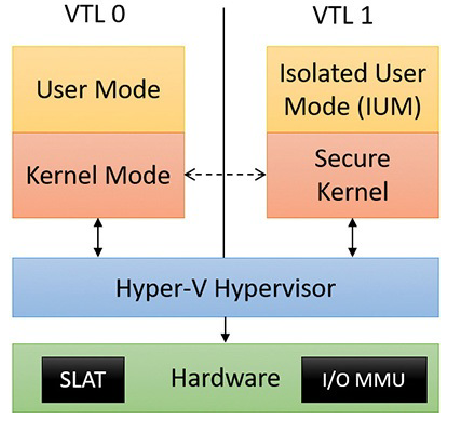
\includegraphics[width=\linewidth]{knowledge/internals/images/vbs-archi.png}
    \caption{VBS architecture}
    \label{fig:vbs_archi}
\end{figure}

\begin{figure}[!ht]
    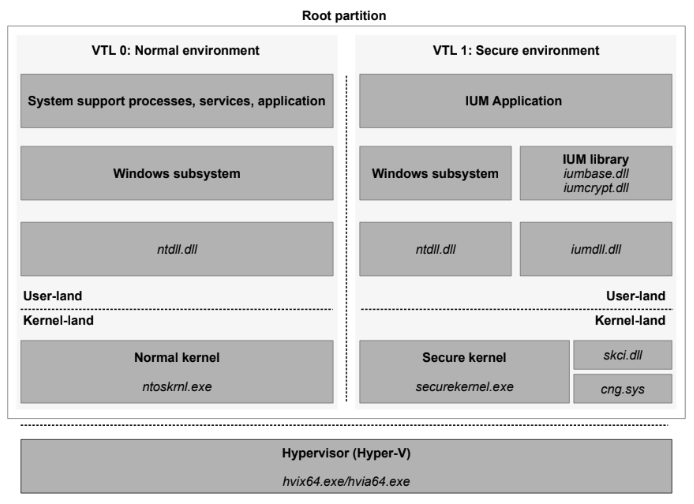
\includegraphics[width=\linewidth]{knowledge/internals/images/vbs-archi-detailed.png}
    \caption{VBS architecture detils}
    \label{fig:vbs_archi_detailed}
\end{figure}


with VBS:
\begin{itemize}
    \item \verb+VTL0+ kernel-mode code cannot touch \verb+VTL1+ user-mode  
    \item \verb+VTL1+ user-mode code cannot touch \verb+VTL0+ kernel-mode 
    \item \verb+\verb+VTL1++ user-mode applications must still go through regular Windows system calls and their respective access checks if they wish to access resources.
\end{itemize}

{\bf copy-on-write mechanisms, prevent \verb+VTL0+ applications from making changes to binaries used by \verb+VTL1+.}

The {\bf secure kernel (\verb+securekernel.exe+)} (aka {\emph proxy kernel}):
\begin{itemize}
    \item does not implement a full range of system capabilities, it hand-picks which system calls it will forward to the \verb+VTL0+ kernel. Any kind of I/O, including file, network, and registry-based, is completely prohibited. Graphics, as another example, are out of the question.
    \item have complete access to \verb+VTL0+ memory and resources
    \item limit the \verb+VTL0+ OS access to certain memory locations by leveraging CPU hardware support known as {\bf Second Level Address Translation (SLAT)}
    (SLAT).
\end{itemize} 

It can leverage:
\begin{itemize}
    \item {\bf Second Level Address Translation (SLAT)}:
        \begin{itemize}
            \item to limit the \verb+VTL0+ OS access to certain memory locations ({\bf Credential guard})
            \item nterdict and control execution of memory ({\bf Device Guard}) locations
        \end{itemize}
    \item {\bf I/O memory management unit (MMU)} which effectively virtualizes memory access for devices to prevent normal device drivers from leveraging hardware devices to directly access memory. This can be used to prevent device drivers from using direct memory access (DMA) to directly access the hypervisor or secure kernel’s physical regions of memory. This would bypass SLAT because no virtual memory is involved.
\end{itemize}

Because the hypervisor is the first system component to be launched by the boot loader, it can program the SLAT and I/O MMU as it sees fit, defining the \verb+VTL0+ and 1 execution environments. Then, while in \verb+VTL1+, the boot loader runs again, loading the secure kernel, which can configure the system further to its needs. Only then is the VTL dropped, which will see the execution of the normal kernel, now living in its \verb+VTL0+ jail, unable to escape.


Only a special class of specially {\bf signed binaries}, called {\bf Trustlets}, are allowed to execute in \verb+VTL1+. 
\begin{itemize}
    \item Each Trustlet has a unique identifier and signature
    \item the secure kernel has hard-coded knowledge of which Trustlets have been created so far
\end{itemize}

As such, it is impossible to create new Trustlets without access to the secure kernel and existing Trustlets cannot be patched in any way.

{\bf IUM}, it’s both:
\begin{itemize}
    \item an environment that restricts the allowed system calls that regular user-mode DLLs can make (thus limiting which of these DLLs can be loaded) 
    \item a framework that adds special secure system calls that can execute only under \verb+VTL1+. 
\end{itemize}    

These additional system calls are exposed in a similar way as regular system calls:
\begin{itemize}
    \item \verb+Iumdll.dll+: The IUM Native Layer DLL implements the secure system call stub. It’s the equivalent of \verb+Ntdll.dll+ of \verb+VTL0+.
    \item \verb+IumCrypt.dll+: Exposes public/private key encryption functions used for signing and integrity verification. Most of the crypto functions exposed to \verb+VTL1+ are implemented in \verb+Iumbase.dll+; only a small number of specialized encryption routines are implemented in \verb+IumCrypt+. \verb+LsaIso+ is the main consumer of the services exposed by \verb+IumCrypt+, which is not loaded in many other trustlets.
    \item \verb+Iumbase.dll+ The IUM Base Layer DLL is the library that implements most of the secure APIs that can be consumed exclusively by \verb+VTL1+ software. It provides various services to each secure process, like secure identification, communication, cryptography, and secure memory management. Trustlets do not usually call secure system calls directly, but they pass through \verb+Iumbase.dll+, which is the equivalent of \verb+kernelbase.dll+ in \verb+VTL0+.
\end{itemize}

A trustlet can be designed to run both in \verb+VTL1+ and \verb+VTL0+. In that case, it should only use routines implemented in the standard \verb+VTL0+ API surface since all the services available to \verb+VTL0+ are also implemented in \verb+VTL1+. For example, a trustlet can never do any registry I/O and any file I/O, but it can use synchronization routines, ALPC, thread APIs, and structured exception handling, and it can manage virtual memory and section objects. Almost all the services offered by the \verb+kernelbase+ and \verb+kernel32+ libraries perform system calls through \verb+Ntdll.dll+. In \verb+VTL1+, these kinds of system calls are {\emph translated} in normal calls and redirected to the \verb+VTL0+ kernel. Normal calls are often used by IUM functions and by the Secure Kernel itself. This explains why \verb+ntdll.dll+ is always mapped in every trustlet.



\subsection{Trustlet}




\subsection{Credential Guard}

Chapter 7

while RunAsPPL protection does guard the NT one-way function (NTOWF) and  TGT key from user-mode attackers, it does not protect against kernel attackers or user-mode attackers that
leverage vulnerabilities drivers.

Credential Guard solves this problem by using another process, \verb+Lsaiso.exe+, which runs as a Trustlet. This process therefore stores the user’s s secrets in its memory, not in \verb+Lsass+.

As \verb+VTL1+ does not have any drivers or access to I/O of hardware of any kind, Isolated LSA cannot directly communicate with the other servers (KDC,\ldots). This is still the responsibility of the Lsass process.

This seemingly results in a problem: the TGT and its key/NTOWF transiently pass through Lsass during authentication, and the TGT and its key are somehow available to Lsass for the generation of service tickets.

This leads to two questions: How does Lsass send and receive the secrets from isolated ISA, and how can we prevent an attacker from doing the same?

To answer the first question, recall that Chapter 3, “Processes and jobs,” described which services are available to Trustlets. One was the Advanced Local Procedure Call (ALPC), which the Secure Kernel supports by proxying the \verb+NtAlpc*+ calls to the Normal Kernel. Then, the Isolated User Mode nvironment implements support for the RPC runtime library (Rpcrt4.dll) over the ALPC protocol, which allows a VTL 0 and VTL 1 application to communicate using local RPC just like any other application and service.


To answer the first question, Although Lsass sits in the middle as a proxy would, it only
sees encrypted traffic between the KDC and isolated LSA, without the ability to understand its contents.

Isolated LSA establishes a {\bf local session key}, which only lives in \verb+VTL1+, and then uses a secure protocol to send this session key encrypted with yet another key (user NTLM ?), which only the KDC has.

The KDC can then respond with the TGT and its key after encrypting it with the isolated LSA session key. Therefore, Lsass sees an encrypted message to the KDC (which it can’t decrypt) and an encrypted message from the KDC (which it can’t decrypt).


Because disabling Credential Guard (which is ultimately nothing more than a registry setting) is trivial for an attacker, Secure Boot and UEFI can be leveraged to prevent a non-physically present administrator from disabling Credential Guard.



\href{https://learn.microsoft.com/fr-fr/windows/security/identity-protection/credential-guard/how-it-works}{Fonctionnement de Credential Guard}

\href{https://learn.microsoft.com/fr-fr/windows/security/identity-protection/credential-guard/considerations-known-issues}{Considérations et problèmes connus liés à l’utilisation de Credential Guard}


\href{https://learn.microsoft.com/fr-fr/windows/security/identity-protection/remote-credential-guard?tabs=intune}{Protection des informations d’identification à distance}
\begin{itemize}
    \item \href{https://github.com/wh0amitz/BypassCredGuard}{Credential Guard Bypass Via Patching Wdigest Memory}
    \item \href{https://itm4n.github.io/credential-guard-bypass/}{Revisiting a Credential Guard Bypass}
\end{itemize}

